\section{Grenzen und Fehler}
\label{sec:Grenzen}

\subsection{Grenzen}
Ein diskretes Halbleiterelement hat immer eine maximale Leistung (meist als $P_{tot}$ bezeichnet), die es umsetzten kann.
Im Fall unseres beliebten IRFP450 sind dies $P_{tot} = \SI{190}{\watt}$ 
\footnote{Im Datenblatt des IRFP450 \cite{IRFP450} als $P_{D}$ bezeichnet}. 
Das Beispiel \ref{sec:Bsp} ist noch innerhalb dieses Wertes 
($P_{Q1} \approx I_{L,max} \cdot U_{L,max} \approx \SI{7}{\ampere} \cdot \SI{20}{\volt} \approx \SI{140}{\watt}$). 
Wenn alles aus diesem MOSFET raus geholt werden soll, übersteigt $P_{Q1}$ schnell $P_{tot}$.

\begin{figure}[h]
	\centering
	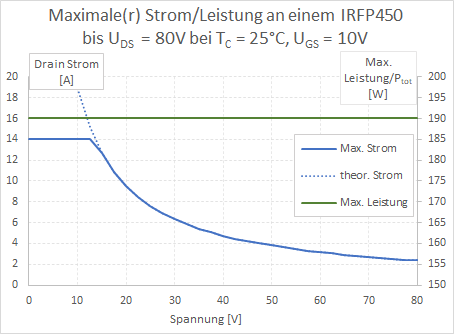
\includegraphics[width=0.5\textwidth]{Bilder/Irfp450_Strom_Spannung.png}
	\renewcommand*\figurename{Diagramm}
	\caption{Maximaler Strom in Abhängigkeit der Spannung unter Berücksichtigung von $P_{tot}$ an einem 
		IRFP450 \cite{IRFP450}}
	\label{dia:IRFP450_S_S_L}
\end{figure}
 
Im Diagramm \ref{dia:IRFP450_S_S_L} ist der Zusammenhang von maximalem Strom gegenüber der Spannung aufgezeigt. 
Der therotische Strom ist dabei über $P_{tot}$ berechnet.
Ein MOSFET-Halbleiter besitzt einen maximalen Drain-Strom, der ebenfalls beachtet werden muss.
Bei dem IRFP450 sind dies 14 Ampere\footnote{$T_{C} = $ 25°C und $U_{GS} = \SI{10}{\volt}$}.
Es ergibt sich die blaue Kurve (Max. Strom). $U_{DS,Q1}$ und $I_{D,Q1}$ darf jeden Wert unterhalb dieser Kurve annehmen. 
Oberhalb würde 
$P_{tot}$ überschritten werden. Gegen diesen Fehlerfall ist die Schaltung nicht gesichert.

\subsection{Fehlerrechnung}

Zu einer Schaltung sind deren Fehler stets anzugeben.
So werden folgend die Fehler und Beispielwerte aufgezeigt.
Die Schaltung der Widerstände $R4$ bis $R2$ werden hier nicht betrachtet, da die Referenzeinstellung über einem \grqq normalen\grqq{} 
Potentiometer eine reine Abschätzung ist und nach einer Anzeige eingestellt werden soll.
Für diese Anzeige sind die Schaltung \ref{sch:OP_Verstärkung}.1/.2 zuständig und werden folgend auf 
ihre Fehler untersucht.
Elektromagnetische Störungen werden ebenfalls nicht betrachtet da diese wie nach Abschnitt \ref{sec:EMV} 
stark minimiert werden können/sollten.\\

Der nicht-invertierende Verstärker macht hier den Anfang.
Neben den weit bekannten und oft schnell ersichtlichen Widerstandstoleranzen, sind die Operationsverstärkereingänge mit 
Eingangsströmen belastet. Diese können hinein oder heraus fließen und werden \textit{Input Bias Current} ($I_{B}$) genannt.
Somit kann eine Spannung am Ausgang der nicht-invertierenden Schaltung \ref{sch:OP_Verstärkung}.1 anliegen, 
ohne das durch $R1$ Strom fließt.  

\begin{equation}
	\Delta U_{R1,IB,ninv} = \biggl(1 + \frac{R11}{R10}\biggr) \cdot R10 \cdot I_{B}
\end{equation}

Neben diesem Fehler gibt es noch die Offset-Spannung. Diese beschreibt die mögliche Spannungsdifferenz 
zwischen den beiden Eingängen (+,-) und wird bei Verstärkung um diese verstärkt. 
Für die nicht-invertierende Schaltung gilt $V_{ges} = V_{U4}$.

\begin{equation}
	\label{eq:Delta_UOffset}
	\Delta U_{Offset} = U_{Offset} \cdot V_{ges}
\end{equation}

Nach der gauß´schen Fehlerfortpflanzung wird die Ausgangsgleichung partiell nach allen Fehlern abgeleitet und addiert.
Nach einsetzen der Formel \ref{eq:V*U_R1} (Ausgangsspannung des nicht-invertierenden Verstärkers) 
ergibt sich die Formel \ref{eq:ninv_Delta_V*U_R1} als Fehler der Verstärkerschaltung. 
Die zusätzlichen Offset- und Eingangsstrom-Fehler des Operationsverstärkers werden addiert. 

\begin{equation}
	\label{eq:V*U_R1}
	U_{R1,ninv} = \biggl(1 + \frac{R11}{R10}\biggr) \cdot R1 \cdot I_{L,max}
\end{equation}

\begin{multline}
	\label{eq:ninv_Delta_V*U_R1}
	\begin{split}
		\Delta U_{R1,ninv,max} 
						=&  \biggl( \biggl| \frac{\delta U_{R1,ninv}}{\delta R11} \biggr| \cdot \Delta R11 \biggr) \\ &+
							\biggl( \biggl| \frac{\delta U_{R1,ninv}}{\delta R10} \biggr| \cdot \Delta R10 \biggr) \\ &+ 
						 	\biggl( \biggl| \frac{\delta U_{R1,ninv}}{\delta R1}  \biggr| \cdot \Delta R1_{max} \biggr) \\ &+
							\Delta U_{R1,IB,ninv} + \Delta U_{Offset}\\
						=&  
							\biggl( \frac{R11}{R10^2} \cdot U_{R1,max} \cdot \Delta R10 \biggr) \\ &+ 
							\biggl( \frac{1}{R10} \cdot U_{R1,max} \cdot \Delta R11 \biggr) \\ &+
							\biggl( \biggl( 1 +\frac{R11}{R10}\biggr)\cdot I_{L,max} \cdot \Delta R1_{max} \biggr) \\ &+
							\Delta U_{R1,IB,ninv} + \Delta U_{Offset}\\
	\end{split}
\end{multline}


Die Toleranz ist von der OP Schaltung abhängig. Für den invertierenden Verstärker (Schaltung \ref{sch:OP_Verstärkung}.2) 
ergibt sich, ebenfalls nach der gauß´schen Fehlerfortpflanzung und Addition der Operationsverstärkerfehler, vereinfacht:

\begin{multline}
	\label{eq:inv_Delta_V*U_R1}
	\begin{split}
		\Delta U_{R1,inv,max} 
						=&  \biggl( \biggl(V_{U3} \cdot \frac{R7}{R6^2} \biggr) \cdot U_{R1,max} \cdot \Delta R6 \biggr) \\ &+
							\biggl( \biggl(V_{U3} \cdot \frac{1}{R6} \biggr) \cdot U_{R1,max} \cdot \Delta R7 \biggr) \\ &+ 
							\biggl( \biggl(V_{U2} \cdot \frac{R9}{R8^2} \biggr) \cdot U_{R1,max} \cdot \Delta R8 \biggr) \\ &+
							\biggl( \biggl(V_{U2} \cdot \frac{1}{R8} \biggr) \cdot U_{R1,max} \cdot \Delta R9 \biggr) \\ &+
							\biggl(V_{ges} \cdot I_{L,max} \cdot \Delta R1_{max} \biggr) \\ &+									% Fertig
							2 \cdot \Delta U_{R1,IB,inv} + 																		% Fertig
							2 \cdot \Delta U_{Offset}\\
	\end{split}
\end{multline}


In der Formel (\ref{eq:inv_Delta_V*U_R1}) darf es $2 \cdot \Delta U_{R1,IB,inv}$ heißen wenn $R6 = R8$.
Wenn nicht, wird $\Delta U_{R1,IB,inv}$ nach Formel \ref{eq:inv_Delta_IB} berechnet und darf in Formel \ref{eq:inv_Delta_V*U_R1} 
nicht mit zwei multipliziert werden.

\begin{equation}
	\label{eq:inv_Delta_IB}
	\Delta U_{R1,IB,inv} = (V_{ges} \cdot R6 \cdot I_{B}) + (V_{ges} \cdot R8 \cdot I_{B})
\end{equation}

Um den Fehler im gesamten Spannungsbereich $U_{R1}$ anzugeben zu können, müssen diese einzeln in 
lineare und absolute Fehler eingeteilt werden. 
Die Fehler $\Delta U_{Offset}$ und $\Delta U_{R1,IB}$ sind absolut und können bei einem Strom 
$I_{L} = \SI{0}{\ampere}$ auftreten.
Die restlichen sind lineare Fehler und von der aktuellen Spannung $U_{R1}$ abhängig. 
Die Formel \ref{eq:+-U_R1} gibt die Spannung plus minus den Fehler zu jener an.

\begin{equation}
	\label{eq:+-U_R1}
	\begin{split}
		U_{R1,(n)inv} \pm \bigg(&\sum \Delta U_{R1,absolut} \\
		&+ \frac{U_{R1,(n)inv}}{U_{R1,(n)inv,max}} \Big(\sum \Delta U_{R1,linear} \Big) \bigg)
	\end{split}
\end{equation}


\subsection{Beispiel für Fehler}

Als Beispiel sind hier die Fehler für beide Schaltungen (nach Tabelle \ref{tab:Werte_Fehler_Beispiel}, 
Seite \pageref{tab:Werte_Fehler_Beispiel} und \ref{tab:Fehler_Beispiel}) 
berechnet. Als Operationsverstärker wurde der LTC2057 \cite{LTC2057} angenommen. 
Das Beispiel aus \ref{sec:Bsp} ist Grundlage für dies ($I_{L,max} = \SI{7}{\ampere}$ usw.). 
Die maximale Temperatur für $R1$ wurde mit \SI{+60}{\degreeCelsius} empirisch festgelegt.

\begin{table}[!h]
	\centering
	\caption{Resultierende Fehler}
	\label{tab:Fehler_Beispiel}
	\normalsize
	\begin{tabular}{l|l|l|c}
		Fehlertyp & linear/ & Term &  Resultierender  \\
				  & absolut && Fehler\\
		\hline
	 	Allgemeine 		& linear 	& $\Delta R1$  				& 21,3 mV \\
						& absolut	& $\Delta U_{Offset}$		& 0,018 mV \\
		\hline
		N. Invertierend & linear 	& $\Delta R10$ 				& 21 mV \\
						& linear 	& $\Delta R11$ 				& 21 mV\\
						& absolut	& $\Delta U_{R1,IB,ninv}$	& 0,03 mV \\
		\hline
		Invertierend 	& linear 	& $\Delta R6$ 				& 28 mV\\
						& linear 	& $\Delta R7$ 				& 28 mV \\
						& linear	& $\Delta R8$ 				& 112 mV\\
						& linear	& $\Delta R9$ 				& 7 mV \\
						& absolut	& $\Delta U_{R1,IB,inv}$	& 0,01 mV \\
		
	\end{tabular}
\end{table}

Die Werte werden in Formel \ref{eq:+-U_R1} wie folgt eingetragen.
\begin{equation}
		U_{R1,ninv} \pm \bigg(0,048 mV
		+ \frac{U_{R1,ninv} \cdot 63,3mV}{2,8V}  \bigg)
\end{equation}

\begin{equation}
	U_{R1,inv} \pm \bigg(0,038 mV
	+ \frac{U_{R1,ninv} \cdot 196,3mV}{2,8V}  \bigg)
\end{equation}

An den Ausgängen der Schaltungen ergeben sich die maximalen Spannungen $U_{R1,ninv,max} = $ 2,8 V $\pm$ 0,063 V und 
$U_{R1,inv,max} = $ 2,8 V $\pm$ 0,196 V. 

In Tabelle \ref{tab:Fehler_Beispiel} ist zu erkennen, dass die Fehler des Input Bias Current und der Offset Spannung sehr klein sind.